\section{Thermodynamics}
(KIILDER)

The free energy\footnote{As we are in the grand canonical ensemble, this is the \emph{grand canonical} free energy, and not Helmholtz' free energy.}
is defined as
\begin{equation}
    \label{thermodynamic free energy}
    F = U - TS - \mu_I Q_I, \quad \dd F = - S \dd T - P \dd V - Q_I \dd \mu_I ,
\end{equation}
where $Q_I$ is the isospin charge, and $U$ is the energy.
As we have seen earlier, our system is homogenous.
This means that the free energy density is independent of volume, and thus $F = V \Ef$.
From  \cref{thermodynamic free energy} we see that the pressure is given by
\begin{equation}
    P = - \left(\diffp{F}{V}\right)_{T, \mu_I} = - \Ef.
\end{equation}
We are interested in the pressure relative to the state in which $\mu_I$ = 0. We therefore normalize $P(\mu_I=0) = 0$, which gives  
\begin{equation}
    P(\mu_I) = -(\Ef(\mu_I) - \Ef(\mu_I = 0))
\end{equation}
This is illustrated in \autoref{fig:pressure}.
\begin{figure}[h]
    \centering
    \vspace{-0.2cm}
    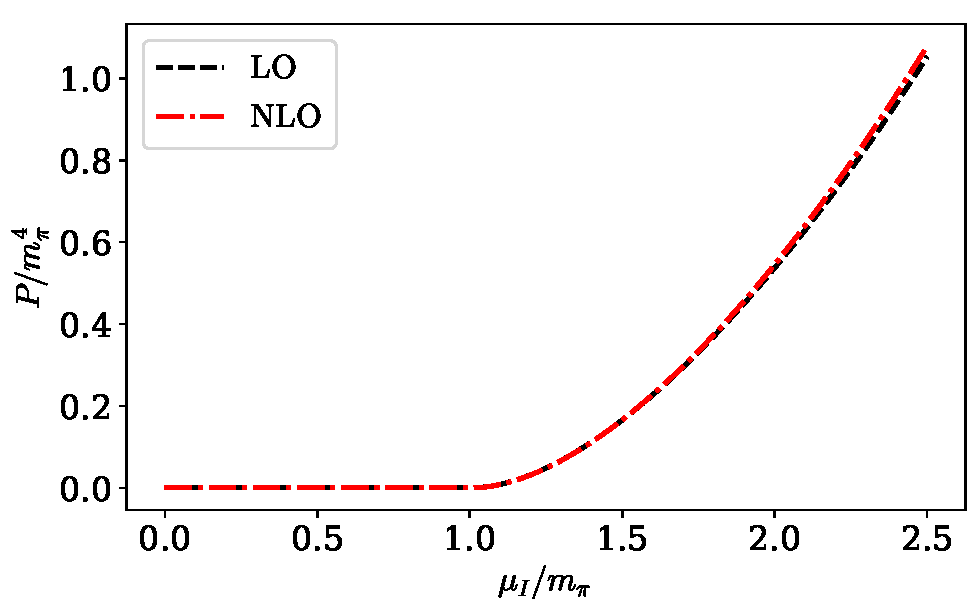
\includegraphics[width=0.7\textwidth]{figurer/numerics/pressure.pdf}
    \caption{The NLO and LO result for the pressure of the pions, as a function of $\mu_I$.}
    \label{fig:pressure}
\end{figure}

Likewise, the total isospin is proportional to volume, which means that the isospin density is
\begin{equation}
    n_I = \frac{Q_I}{V} = - \frac{1}{V} \left(\diffp{F}{\mu_I}\right)_{T, V}
    = - \diffp{\Ef}{\mu_I}.
\end{equation}
This gives 
\begin{align}
    \nonumber
    n_I & = 
    f^2 \mu_I \sin^2 \alpha
    - \diffp{\Ef_\mathrm{fin}}{\mu_I} \\
    & + \frac{1}{(4 \pi)^2}
    \left[
            \left(2\bar l_4+\ln\frac{M^2}{m_3^2}\right)\bar m^2 \mu_I \cos\alpha \sin^2 \alpha
            +\frac{1}{3}\left(2\bar l_1 + 4 \bar l_2 + 3\ln\frac{M^2}{m_3^2}\right)\mu_I^3 \sin^4 \alpha
    \right]
\end{align}
The isospin density, as a function of $\mu_I$, is shown in \autoref{fig:isospin_density}.
\begin{figure}[!h]
    \centering
    \vspace{-0.2cm}
    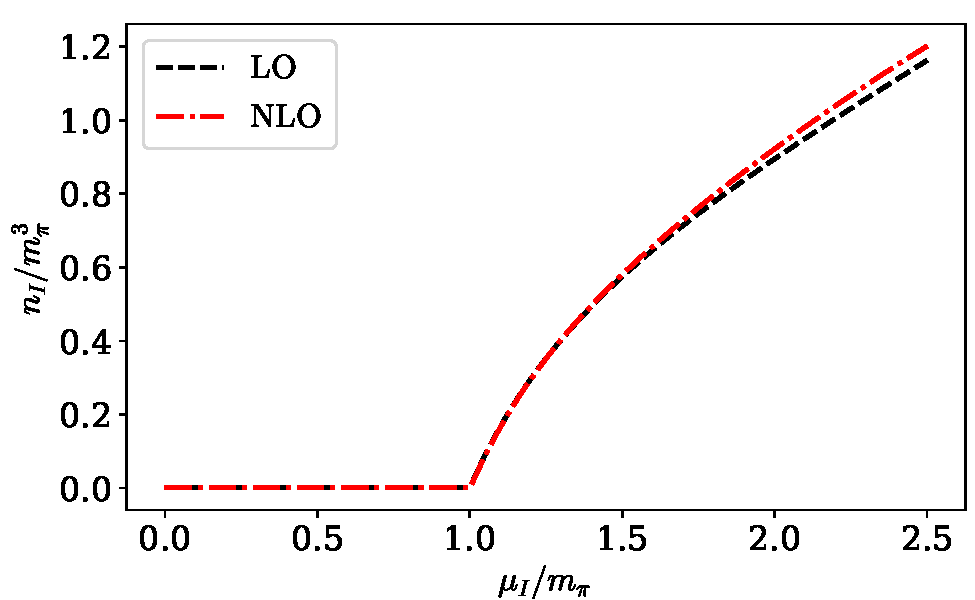
\includegraphics[width=0.7\textwidth]{figurer/numerics/isospin_density.pdf}
    \caption{The NLO and LO result for the isosopin densisty, as a function of $\mu_I$.}
    \label{fig:isospin_density}
\end{figure}

From \cref{thermodynamic free energy} we get the energy density, $u = U/V$, at $T = 0$ is given by
\begin{equation}
    u(\mu_I) = -P(\mu_I) + \mu_I n_I(\mu_I),
\end{equation}
where we again have normalized so that $u(\mu_I = 0) = 0$.
Now that we have both the dependence of pressure and energy density on the isospin chemical potential, we can trace out the line in the pressure-energy density plane, parametrized by $\mu_I$.
This is shown in \autoref{fig:equation of state}.
This is the equation of state of the system.

\begin{figure}[!h]
    \centering
    \vspace{-0.2cm}
    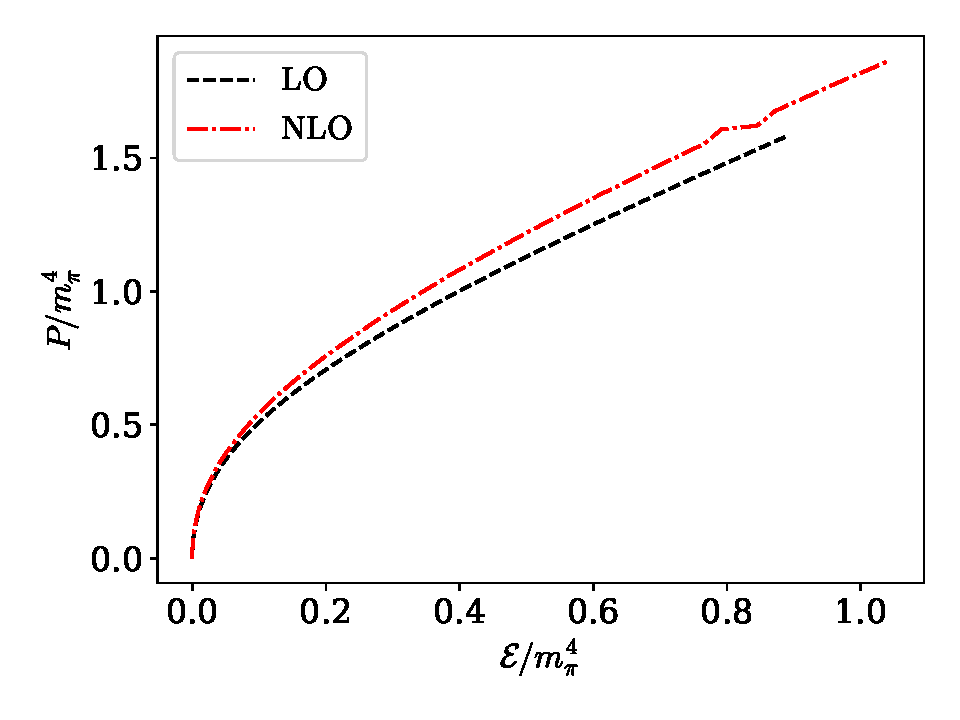
\includegraphics[width=0.7\textwidth]{figurer/numerics/energy_density.pdf}
    \caption{The equation of state of the system.}
    \label{fig:equation of state}
\end{figure}

\FloatBarrier

\subsection*{Phase transition}
(KILDER)

In our leading-order analysis, we saw that $\alpha$ was zero for $\mu_I \leq \bar m$, before it starts to increase for $\mu_I>\bar m$, and that $\bar = m_\pi$.
The behavior of $\alpha$ is illustrated in \autoref{fig:alpha}.
This is the hallmark of a phase transition, where $\alpha$ is the order parameter.
The behavior systems near points of phase transition is described by Landau theory.
Using \cref{leading order contribution free energy}, we can expand the leading-order free energy in $\alpha$,
\begin{align}
    \Ef
    & = -f^2 \bar m^2 + f^2 \frac{1}{2}(\bar m^2 - \mu_I^2)\alpha^2
    - \frac{1}{24} f^2 (\bar m^2 - 4 \mu_I^2) \alpha^4 + \Oh[5]{\alpha} \\
    & = \Ef(\alpha=0) + a(\mu_I)\alpha^2 + \frac{1}{2} b(\mu_I)\alpha^4 + \Oh[5]{\alpha},
\end{align}
to leading order.
Notice that near $\mu_I = \bar m$, $b > 0$.
As earlier, the equation that governs $\alpha'$ is
\begin{equation}
    \label{landau ginsburg lo}
    \diffp{\Ef}{\alpha} \bigg|_{\alpha=\alpha'} = 2 [a(\mu_I) + b(\mu_I) \alpha^2] \alpha = 0.
\end{equation}
If $a>0$, then $\alpha' = 0$ will be the only solution, which gives us the criterion for a phase transition 
\begin{equation}
    a(\mu_I) = 0,
\end{equation}
which again gives $\mu_I = \bar m$.
Near $\mu_I = \bar m$, we can write
\begin{equation}
    a = - a_0 (\mu_I - \bar m), \quad b = b_0,
\end{equation}
where $a_0$ and $b_0$ are positive constants, so the solution to \cref{landau ginsburg lo} for $\mu_I>\bar m$
\begin{equation}
    \alpha(\mu_I) = \sqrt{\frac{a_0}{b_0}} (\mu_I - \bar m)^{1/2}.
\end{equation}
The order parameter $\alpha$ changes continuously as the system undergoes phase-transition.
This means we have a \emph{second order} phase transition.
However, if $b < 1$ near $\mu_I = \bar m$, this is not a valid solution, so we must expand $\Ef$ further to show if the phase transition is continuous or not.
The difference is illustrated in \autoref{fig:phase transition}.
\begin{figure}
    \centering
    \begin{subfigure}{0.49\textwidth}
        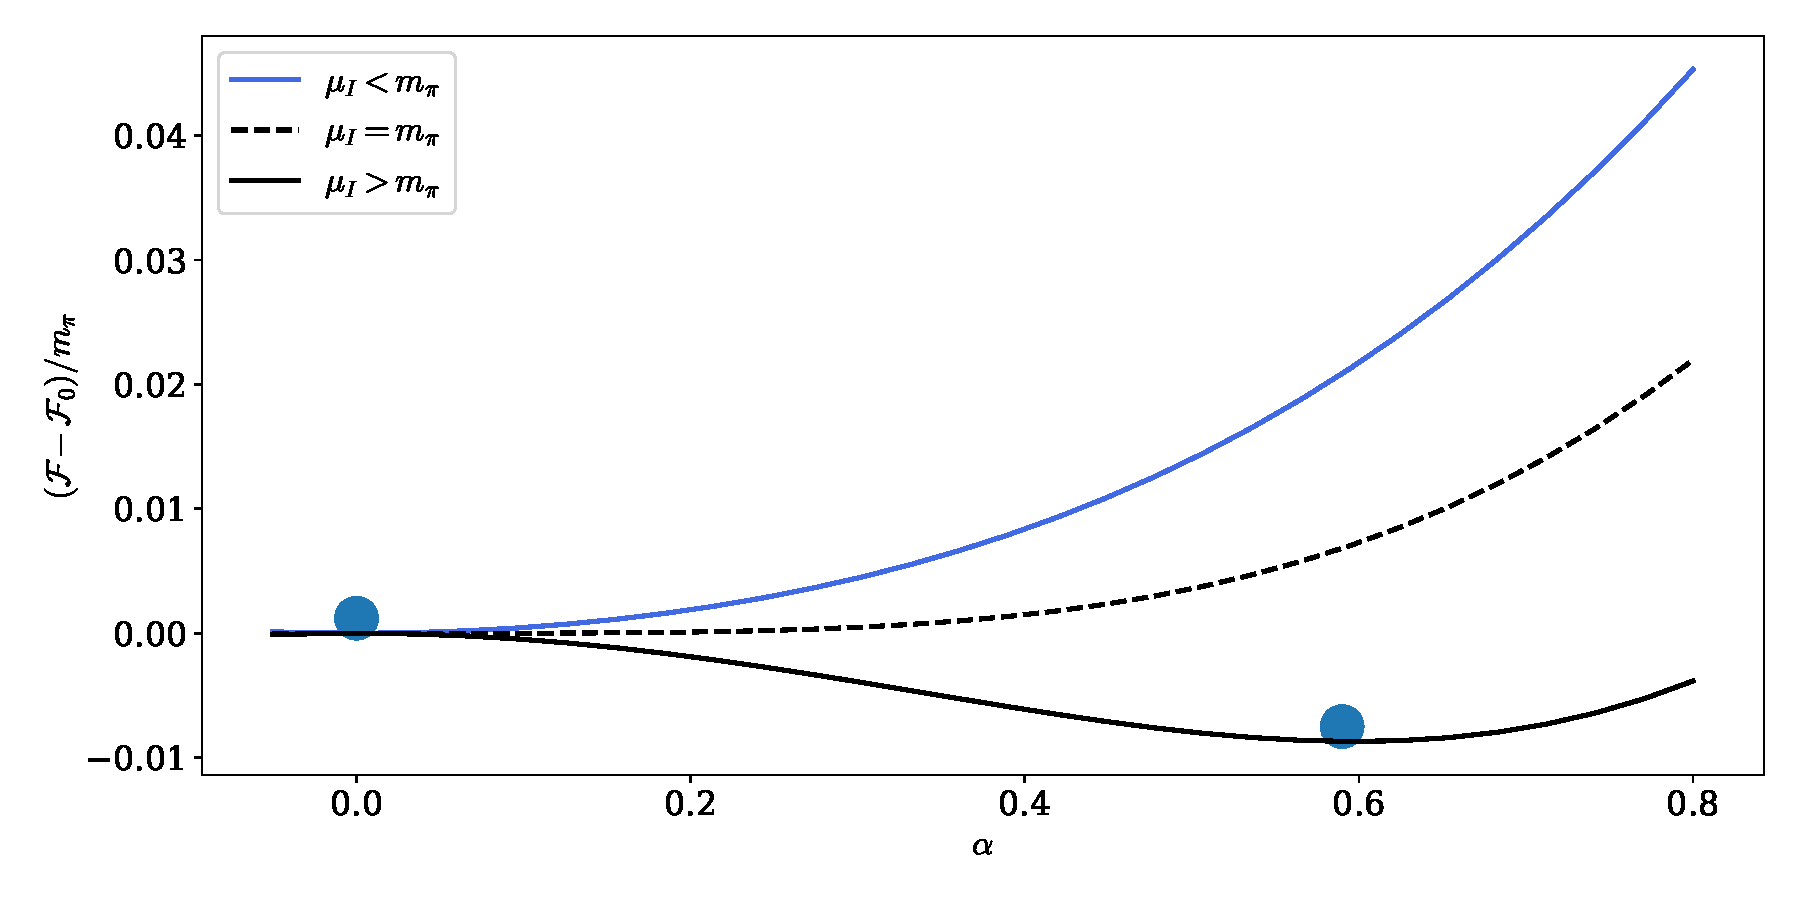
\includegraphics[width=\textwidth]{figurer/numerics/phase_transition.pdf}
    \end{subfigure}
    \begin{subfigure}{0.49\textwidth}
        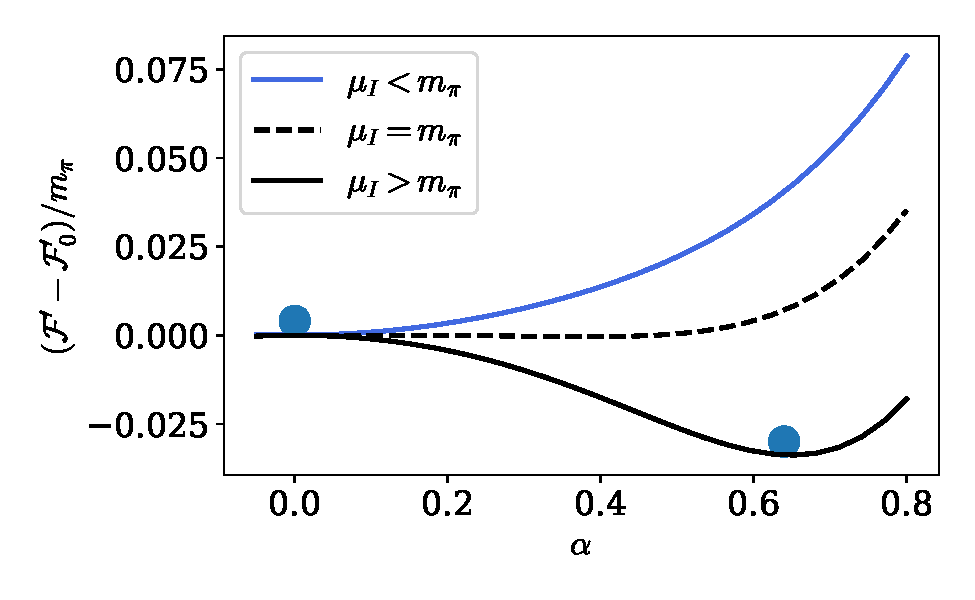
\includegraphics[width=\textwidth]{figurer/numerics/phase_transition2.pdf}
    \end{subfigure}
    \caption{The plot on the left shows normalized free energy density as a function of $\alpha$, in the two different phases. The plot on the right shows the same, but with a free energy $\Ef'$ that have been modified so that $b(\mu_I=\bar m)<0$.
    In the first case, the minima transitions continuous, while in the second it jumps.}
    \label{fig:phase transition}
\end{figure}

% Due to symmetry of the system under $\alpha \rightarrow -\alpha$, the expansion of $\Ef$ should only contain even powers.
% This can be certified to leading order by explicit calculation.
% We therefore write,
% \begin{equation}
%     \Ef = \Ef(\alpha = 0) + a \alpha^2 - \frac{1}{2} b \alpha^4 + \frac{1}{3} c \alpha^6
%     + \Oh[8]{\alpha}.
% \end{equation}
% We assume that near $\bar m = \mu_I$, we can write $a = -a_0(\mu_I - \bar m), \, b = -b0 ,½$ and $c = c_0$, where all the constants are positive.
% The equation for $\alpha'$ is now
% \begin{equation}
%     2\alpha [a - \alpha^3 (b - c \alpha^3 )] = 0
% \end{equation}
% We still have the $\alpha' = 0$ for $\mu_I < \bar m$.
% For $\mu_I> \bar m$, we get the solutions
% \begin{equation}
%     \alpha^3 = \frac{1}{2} \left( \frac{b}{c} \pm \sqrt{\left(\frac{b}{c} \right)^2- 4 \frac{a}{c}} \right)
%     = \frac{b_0}{2c_0} \left(1 \pm \sqrt{1- 4 (\mu_I - \bar m) \frac{a_0c_0}{b_0^2}} \right).
% \end{equation}
% Taking the second derivative, 
% \begin{equation}
%     \Ef' = a - (3 b - 5c \alpha^2)\alpha^2,
% \end{equation}



In the vacuum phase, $\alpha' = 0$, the ground state is given by 
\begin{equation}
    \Sigma(\pi = 0) = \Sigma_0 = \one,
\end{equation}
where we have use \cref{sigma}.
Under $H = SU(2)_V$, $\Sigma$ transforms as
\begin{equation}
    \Sigma(x) \rightarrow \Sigma'(x) = V \Sigma(x) V^\dagger,
    \quad
    V = \exp{i \theta_a \tau_a},
\end{equation}
which means that the vacuum phase ground state is invariant under $H$.
However, for $\alpha = 0$, the ground state is shifted to
\begin{equation}
    \Sigma(\pi=0) = A_\alpha \Sigma_0 A_\alpha = \exp{i \alpha \tau_1}.
\end{equation}
The generators $\tau_2$ and $\tau_3$ are broken.
The new ground state corresponds to a condensate of the $\pi_1$-particle, as it is defined in the vacuum state.
In \autoref{fig:masses}, we saw that the mass of the $m_-$ particle vanishes, so we identify this particle with the corresponding Goldstone mode.
There is only one Goldstone mode, however this is not a Lorentz invariant system, in which case we cannot guarantee one massless mode per broken generator. (ER DETTE RIKTIG?)

To find the value of $\mu_I$ to next-to-leading order, we must expand the NLO free energy in powers of $\alpha$
When we expand the static, second order Lagrangian to $\alpha^2$, we get
\begin{align}
    \Ef_4^{(0)}
    &= - (l_3 + l_4)\bar m^4 + [(l_3 + l_4)\bar m^4 -l_4 \bar m^2\mu_I^2]\alpha^2
    % \\
    % &
    % = \mu^{-2\epsilon} \frac{1}{(4\pi)^2}
    % \left[
    %     \left(
    %         -\frac{1}{4}(\bar l_3 - 1 - \frac{1}{\epsilon} - \ln\frac{\tilde \mu^2}{M^2})
    %         + (\bar l_4 - 1 - \frac{1}{\epsilon} - \ln\frac{\tilde \mu^2}{M^2})
    %     \right)\bar m^4
    %     -(\bar l_4 - 1 - \frac{1}{\epsilon} - \ln\frac{\tilde \mu^2}{M^2}) \bar m^2\mu_I^2
    % \right]\alpha^2
    % + \Oh[3]{\alpha}
    % \\
    % &
    % = \const + \mu^{-2\epsilon} \frac{1}{(4\pi)^2}
    % \left[
    %     \frac{3}{4}
    %     \left(
    %         \frac{4}{3}\bar l_4 - \frac{1}{3}\bar l_3 - 1 - \frac{1}{\epsilon} - \ln\frac{\tilde \mu^2}{M^2}
    %     \right)\bar m^4
    %     -
    %     \left(
    %         \bar l_4 - 1 - \frac{1}{\epsilon} - \ln\frac{\tilde \mu^2}{M^2}
    %     \right) 
    %     \bar m^2\mu_I^2
    % \right]\alpha^2
    % + \Oh[3]{\alpha}
    \\
    & =
    \const + 
    \frac{\mu^{-2\epsilon}}{(4\pi)^2}
    \left[
        \left(
            \bar l_4 - \frac{1}{4}\bar l_3
        \right)\bar m^4
        -\bar l_4\bar m^2\mu_I^2
        -\left(
            1 + \frac{1}{\epsilon} + \ln\frac{\tilde \mu^2}{M^2}
        \right)
        \left(\frac{3}{4}\bar m^2 - \mu_I^2\right)\bar m^2
    \right]\alpha^2,
\end{align}
where $\const$ is independent of $\alpha$, and thus not of interest.
From the one-loop correction, we have the contributions
\begin{equation}
    \Ef_2^{(1)} = i \frac{1}{2}\int \frac{\dd^4 p}{(2\pi)^2} \ln(-p^2 + m_3^2)
    +  i \frac{1}{2} \int \frac{\dd^4 p}{(2\pi)^2} \ln[(-p^2 + m_1^2)(-p^2 + m_2^2) - p_0^2 m_{12}^2]
\end{equation}
% We have already evaluated the first integral when ca
The first integral is the same free energy contribution from the $\pi_0$-particle as we have calculated earlier, and it reads
\begin{equation}
    \Ef_{\pi_0} 
    = i \frac{1}{2}\int \frac{\dd^4 p}{(2\pi)^2} \ln(-p^2 + m_3^2)
    = - \mu^{-2\epsilon}\frac{1}{4} \frac{m_3^4}{(4 \pi)^2}
    \left(\frac{1}{\epsilon} + \frac{3}{2} + \ln \frac{\tilde \mu^2}{m_3^2}\right).
\end{equation}
The mass $m_3$ is dependent on $\alpha$, and has the expansion
\begin{align*}
    % m_3^2 
    % &= \bar m^2 + \frac{1}{2}(2\mu_I^2 - \bar m^2)\alpha^2+ \Oh[3]{\alpha}, \\
    m_3^4
    &= \bar m^4 + \bar m^2(2\mu_I^2 - \bar m^2)\alpha^2+ \Oh[3]{\alpha}, \\
    \ln \frac{\mu^2}{m_3^2}
    &=
    \ln \frac{\mu^2}{\bar m_3^2} - \frac{1}{2} \frac{(2\mu_I^2 - \bar m^2)}{\bar m^2}+ \Oh[3]{\alpha}.
\end{align*}
In the second integral, we rewrite the argument of the logarithm as
\begin{equation}
    (-p^2 + m_1^2)(-p^2 + m_2^2) - p_0^2 m_{12}^2
    =  \left[-p^2 + \frac{1}{2}(m_1^2 + m_2^2)\right]^2 - p_0^2 m_{12}^2 - \frac{1}{4}(m_1^2 - m_2^2)^2.
\end{equation}
When we calculate the $\alpha$ dependence of the last term, we get  $(m_1^2 - m_2^2)^2 = \mu^4 \sin^4\alpha = \Oh[4]{\alpha}$, which means that for our purposes, we can ignore this term.
We further rewrite the remaining expression by factoring it,
\begin{equation}
    \left[-p^2 + \frac{1}{2}(m_1^2 + m_2^2)\right]^2 - p_0^2 m_{12}^2
    = \left[-p^2 + \frac{1}{2}(m_1^2 + m_2^2) - p_0 m_{12} \right]
    \left[-p^2 + \frac{1}{2}(m_1^2 + m_2^2) + p_0 m_{12} \right]
\end{equation}
% Each of these can be brought into a form so that we can perform the integral after a change of variables, through
% With a change of 
We then complete the square in each of the factors,
\begin{equation}
    - p^2 + \frac{1}{2}(m_1^2 + m_2^2) \pm p_0 m_{12}
    = - \left(p_0 \mp \frac{1}{2}m_{12}\right)^2 + |\vv p|^2 + m_4^2,
\end{equation}
where
\begin{align}
    m_4^2 &= \frac{1}{2}\left(m_1^2 +m_2^2 +\frac{1}{2}m_{12}\right)
    % = \bar m^2 \cos\alpha - \frac{1}{2} \mu_I^2 (\cos 2\alpha + \cos^2 \alpha - 2\cos^2\alpha)
    = \bar m^2 \cos\alpha + \frac{1}{2} \mu_I^2 \sin^2 \alpha, \\
    % M^2
    % &= \bar m^2 -\frac{1}{2}(m^2 + \mu_I^2) \alpha^2 + \Oh[3]{\alpha}, \\
    m_4^4
    &= \bar m^4 - \bar m^2(m^2 + \mu_I^2) \alpha^2 + \Oh[3]{\alpha}, \\
    \ln \frac{\mu^2}{m_4^2} 
    &= \ln \frac{\mu_I^2}{\bar m^2} + \frac{1}{2}\frac{\bar m^2 + \mu_I^2}{\bar m^2}\alpha^2
    + \Oh[3]{\alpha}.
\end{align}
After a shift of variables, the integral has the same form as the logarithmic integrals we have calculated earlier, which gives us the result
\begin{equation}
    \Ef_{\pi_\pm}
    = i \int \frac{\dd^4}{(2\pi)^4}
    \ln(-p^2 + M^2)
    = 
    - \mu^{-2\epsilon}\frac{1}{2} \frac{M^4}{(4 \pi)^2}
    \left(\frac{1}{\epsilon} + \frac{3}{2} + \ln \frac{\tilde \mu^2}{M^2}\right)
\end{equation}
Combining these two contributions to the one-loop correction of the free energy gives
\begin{align*}
    \Ef_2^{(1)}
    &=
    \mathrm{const.}
    +
    \frac{\mu^{-2 \epsilon } }{(4 \pi)^2} 
    \left(1 + \frac{1}{\epsilon} + \ln \frac{\tilde \mu^2}{m^2}\right)
    \left(\frac{3}{4}m^2 - \mu_I^2\right)
    \bar m^2 \alpha^2
\end{align*}
We see that again, the $\epsilon^{-1}$ will cancel when we combine the NLO-terms, and we get
\begin{align}
    \tilde \Ef_1
    & = 
    \const+ 
    \frac{1}{(4\pi)^2}
    \left[
        \left(
            \bar l_4 - \frac{1}{4}\bar l_3
        \right)\bar m^4
        -\bar l_4\bar m^2\mu_I^2
        + \ln\frac{M^2}{\bar m^2}
        \left(\frac{3}{4}\bar m^2 - \mu_I^2\right)\bar m^2
    \right]\alpha^2
    + \Oh[3]{\alpha}.
\end{align}
The total NLO free energy, up to second order in $\alpha$, is
(HVOR BLE DET AV LOG? TROR DET ER 1 + HØYERE ORDEN. SJEKK!)
\begin{equation}
    \Ef_{\mathrm{NLO}}
    =
    \Ef_{\mathrm{NLO}}(\alpha = 0)
    +
    \frac{1}{2} f^2 \bar m^2
    \left(
        1
        -
        \frac{1}{2}
        \frac{\bar l_3 - 4 \bar l_4}{(4 \pi)^2} \frac{\bar m^2}{f^2}
    \right)\alpha^2
    - \frac{1}{2}f^2 \mu_I^2
    \left(
        1
        +
        \frac{2 \bar l_4}{(4 \pi)^2}
        \frac{\bar m^2}{f^2}
    \right) \alpha^2
    + \Oh[3]{\alpha}.
\end{equation}
We now insert the physical constants $f_\pi$ and $m_\pi$, by using the next-to-leading order expressions \cref{equation bare mass} and \cref{equation bare decay constant}.
First, notice that
\begin{equation}
    f_\pi^2 m_\pi^2
    = f^2 \bar m^2
    \left(
        1 - \frac{1}{2} \frac{\bar l_3 - 4 \bar l_4}{(4 \pi)^2} \frac{\bar m^2}{f^2}
        +
        \Oh[]{\frac{\bar m^4}{f^4}}
    \right)
\end{equation}
This means that, to leading order,
\begin{equation}
    \Ef_{\mathrm{NLO}}
    =
    \Ef_{\mathrm{NLO}}(\alpha = 0)
    + \frac{1}{2}f_\pi^2 (m_\pi^2 - \mu_I^2 )\alpha^2
    + \Oh[3]{\alpha}.
\end{equation}
This shows that the phase transition happens at $\mu_I = m_\pi$, also at next-to-leading order.
